% This is samplepaper.tex, a sample chapter demonstrating the
% LLNCS macro package for Springer Computer Science proceedings;
% Version 2.20 of 2017/10/04
%
\documentclass[runningheads]{llncs}
%
\usepackage{graphicx}
% Used for displaying a sample figure. If possible, figure files should
% be included in EPS format.
%
% If you use the hyperref package, please uncomment the following line
% to display URLs in blue roman font according to Springer's eBook style:
% \renewcommand\UrlFont{\color{blue}\rmfamily}

\begin{document}
%
\title{NeoMycelia: A software reference architecture for big data systems}
%
%\titlerunning{Abbreviated paper title}
% If the paper title is too long for the running head, you can set
% an abbreviated paper title here
%
\author{Pouya Ataei\inst{1}\orcidID{0000-0002-0993-3574} \and
    Alan Litchfield\inst{1}\orcidID{0000-0002-3876-0940}}
%
\authorrunning{P. Ataei et al.}
% First names are abbreviated in the running head.
% If there are more than two authors, 'et al.' is used.
%
\institute{Auckland University of Technology, Auckland 1010, New Zealand
    \email{\{pataei, alan.litchfield\}@aut.ac.nz}
}
%
\maketitle              % typeset the header of the contribution
%
\begin{abstract}
    The big data revolution began when the volume, velocity, and variety of data completely overwhelmed the systems used to store, manipulate and analyze that data. As a result, a new class of software systems emerged called big data systems. While many attempted to harness the power of these new systems, it is estimated that approximately 75\% of the big data projects have failed within the last decade. One of the root causes of this is software engineering and architecture aspect of these systems. This paper aims to facilitate big data system development by introducing a software reference architecture. The work provides an event driven microservices architecture that addresses specific limitations in current big data reference architectures (RA). The artefact development has followed the principles of empirically grounded RAs. The RA has been evaluated by developing a prototype that solves a real-world problem in practice. At the end, succesful implementation of the reference architecture have been presented. The results displayed a good degree of applicability with respect to quality factors.

    \keywords{Reference architecture \and Architecture \and Big data reference architecture \and Big data architecture \and Big data systems \and Big data software engineering \and Big data and microservices \and Event driven big data systems \and Event driven \and Microservices}
\end{abstract}
%
%
%
\section{Introduction}
The ubiquity of digital devices, the networking infrastructure of today, and the proliferation of software applications, have augmented users’ capability to produce data at an unprecedented rate \cite{AtaeiHype}. In a world where we have an average processing power of 1.5 GHz on smart phones, and up to 8 GHz on laptops running on a network infrastructure that will support up to 25 Mbps of transmission per second, data becomes the new oil, the atom, the dot that lays the foundation of a nexus \cite{Shafi}.

BD is a term that was initially coined to refer to the gradual growth and availability of data \cite{lycett2013datafication}. BD is an endeavor to harness patterns behind vast amounts of data for the purposes of improvement, control, and prediction. Roughly 10 years ago, the BD revolution began when the volume, velocity, and variety of data completely overwhelmed the systems used to store, manipulate and analyze that data \cite{heudecker2014survey,AtaeiBigDataEnvirons}. The concept of BD is a game-changing innovation \cite{chen2017big}, heralds the dawn of a new industrial revolution \cite{Huberty}, and creates a new category of economic asset.

Nevertheless, BD is not always better data or a magic wand that enchants any business or process. Actually, it can very easily cause losses \cite{Ranjan}. It is estimated that approximately 75\% of the BD projects have failed within the last decade according to multiple sources \cite{Partners,analytics2016age,Nash,heudecker2014survey}. Among challenges of adopting BD, the most repeatedly discussed are 1) Architectural and system development challenges, 2) Organizational challenges, and 3) Rapid technology change \cite{chen2017big,AtaeiHype,Singh}. The focus of this study is on architectural and system development challenges.

Today, most BD systems are developed as ad-hoc and complicated architectural solutions that do not tend to adhere to many principles of software engineering \cite{Gorton,Nadal}. In addition, as the ecosystem of big data grows and new technologies are introduced, architects will have harder time to select and orchestrate the right technology to produce the right results \cite{Nadal}.

This can create a foundation for an immature architectural decision that results in a solution that is hard to maintain, hard to scale, and may raise high-entry barriers.  Since the approach of ad-hoc design for BD systems is undesirable and leaves many engineers in the dark, novel software engineering approaches specialized for BD systems are required. To contribute towards this goal, we explore the notion of RAs.

In the case of ambiguity towards what should be developed to address what needs, RA can play an overarching role to describe the building blocks of the system and the ways in which these blocks communicate to achieve the overall goal of the system \cite{Sievi-Korte}. This in turn produces manageable modules that each address a different aspect of the problem, and provides stakeholders with a high-level medium to observe, reflect upon, communicate with and add into.


\section{Why Reference Architectures?}

Big data is an interplay of analytics methods, software engineering through development and data engineering, and organizational workflows \cite{Mannering,Selamat}. Such complex systems are best approached through the lens of architecture and well-thought out design documents. utilization of RAs for complex systems is not something new.

In fact, practitioners of complex systems, software engineers, and system designers have been frequently using reference architectures to have a collective understanding of system components, functionalities, data-flows and patterns which shape the overall qualities of system and help further adjust it to the business objectives \cite{Kohler,Cloutier}. In software product line (SPL) development, reference architectures are generic schemas that can be configured and instantiated for a particular domain of systems \cite{Derras}. In software engineering, reference architecture (RA) can be defined as means to represent and transfer knowledge that bridges from the problem domain to a family of solutions \cite{Klein}.

RAs serve as a mechanism that embodies domain relevant qualities and concepts, breaks down the solutions and generates a terminology to facilitate effective communication, and illuminates various stakeholders and system designers \cite{Klein}. This allows RAs to provide an opportunity for early identification of design issues, when making changes is still cheap. This allows brings about several side-benefits such as:
\begin{enumerate}
    \item Ensuring cross-cutting concerns are addressed
    \item Scales the know of architects and engineers across the organization
    \item Helps achieving consensus around major design choices
    \item Creates the foundation of organization memory around design decisions
    \item Acts as a blueprint and a summary artefact in the portfolio of the architects and software engineers
\end{enumerate}


Many of the prevalent technologies in the industry have stemmed from a RA \cite{Cioroaica}. OATH is a commonly used protocol for authentication over the web and the OATH RA is the result of an industry-wide collaboration using open standards \cite{OATH}. Similarly, the ANSI-SPARC architecture, based on the ANSI-SPARC design standard for database management systems \cite{ANSI}, grew to become common among practitioners.


\section{Research Methodology}


To increase systematicity and allow for reproducibility of Neomycelia, we follow the guidelines presented in empirically-grounded RAs \cite{GALSTER}. In essence, “empirically grounded” implies two major aspects: 1) “empirical foundation” which implies that Neomycelia must be grounded in proven principles (domain problems, practical concepts), and 2) “empirical validity” which implies that RA needs to be evaluated for applicability and validity. This research methodology is based on two main pillars: 1) existing RAs and 2) literature on RAs. The process follows these 6 steps:

\textbf{1. Decision on type of the RA}:  A classification framework presented by \cite{angelov2009classification} is applied. In this study, five types of RAs have been described from which our RA matches type five (facilitation architectures designed to be implemented in multiple organizations). Thus, this RA aims to facilitate the design of big data systems across multiple organizations. Examples of similar RAs are ERA \cite{angelov2008contracting}, AHA \cite{Wu}, and eSRA \cite{norta2014reference}

\textbf{2. Design Strategy}: There are two general approaches to the development of RAs; developing RAs from scratch or from existing architectures. Our RA is developed based on existing architectures and available literatures.

\textbf{3. Empirical acquisition of data}: Data acquisition consists of two major phases, data sources identification and capturing architecture data. It is proposed by Nakagawa (\cite{Nakagawa}) that good data sources for classical RA development can be people (researchers, practitioners), available literature (publications, technical reports, white papers) and systems (source codes, documentations). Howbeit, the guidelines presented by Galster and Avgeriou (\cite{GALSTER}), provide no means or instructions on how these data should be identified and captured.

Therefore, to increase systematicity and transparency of this research, we conducted a systematic literature review to capture current best evidence from the available literature. For this purpose we follow the guidelines of PRISMA presented by Shamseer et al. (\cite{Shamseer}).

Our aim was to find all available big data reference architectures in literature and gray literature. This has helped by grounding a solid formation for development of Neomycelia. We’ve selected IEEE Explore, ScienceDirect, SpringerLink, ACM library, MIS Quarterly, Elsevier, AISel as well as citation databases such as Scopus, Web of Science, Google Scholar, and Research Gate. The search keywords used are Big Data Reference Architectures; Reference Architectures in the domain of Big Data; Reference Architectures and Big Data;

In the first phase of the SLR (identification), 84 literature has been pooled. Out of this pool, 57 study has been selected based on our inclusion, exclusion and quality criteria. Studied that provided with detailed analysis and practice have been included. Studied that provided with substantial case studies have been included. Papers that discussed current BD RAs, it’s ecosystems and drivers have been included. Papers that are recent (in the range of 2010-2020) have been included.

On the other hand, papers that are duplicates, do not directly address the SLR aim, and are not written in English are excluded. For our quality factors, we paid extensive attention to how rich the study is in terms of its case studies and relevance to practice. The length and volume of the information provided by the studies has been considered as well. Very short and information lacking papers did not get pass through the quality assessment framework.

In the pool of selected articles, 24.5\% from SpringerLink, 16\% from ACM, 33\% are from IEEE Explore, 5.2\% from ScienceDirect, and the rest from Google Scholar. 13 conference proceedings, 30 journal articles, 12 book chapters, and a whitepaper has been selected. 33\% belonged to years 2013-2015, 51\% of the articles were selected from the years 2016-2020, and the rest to years 2010-2013.

We used the software Nvivo for and classifying these literatures. We defined 3 nodes namely ‘big data architecture data’, ‘big data reference architecture limitations’, and ‘big data reference components”. Once we coded and attributed texts to our nodes, we then synthesized and inferred findings.

The result of this SLR administered 23 RAs from extant literature, 18 RAs from academia, 4 from practice, 1 through the collaboration of both domains. Majority of the RAs has been in the form of short papers, but there has been few detailed RAs as well. The exact detail and listing of the RAs are out of the scope of this study, however, there will be mention to various RAs for comparison, inference purposes.

We found three common components among all RAs which are; big data management and storage nodes (relational, non-relational, graph, data lake, data finery, polyglot persistence), big data infrastructure nodes (latency, data transformation, in-memory data grids), and big data analytics and application nodes (real-time processing, batch processing, predictive analysis, spatial analysis). This underpinned our understanding for actual design and construction of the RA. The findings from this phase is further elaborated in section 5 of this paper.

4. Construction of the RA: Based on the findings captured in phase 3, the initial design of the RA took place. Integral to this phase, was the underlying method to creation and design of RA. We followed ISO/IEC 42010 for architectural descriptions (Chaabane et al. 2017). The standard mostly revolves around concrete architectures and for that sake, our descriptions do not 100\% conform to it.

For instance, the standard has bolded the identification of system stakeholders (clause 5), however RAs are highly abstract and do not have a clear group of stakeholders (Ataei and Litchfield 2020). Another focal point in conveyance of architectural descriptions is the concept of views. In this case, ISO/IEC 42010, being the standard for concrete architectures, prescribe architecture views and viewpoints in the context of business and actual models (clause 4). This does not apply to this RA as well.

Moreover, Beneken (2018) classified three different kind of RAs based on the views, namely functional, logical and technical. Along the lines, Vogel et al. (2009) classified RAs based on their usage context, as platform-specific, industry specific, industry crosscutting, and product line RAs.

Whereas different academic efforts aimed at classifying RAs based on different criteria, arguably several distinct views can adhere to one logical view as it has been seen in the case of pattern based reference architecture for serviced based system conducted by Stricker et al. (2010). This implies, that modules defined in technical review can potentially refine the modules of the logical view. Cloutier et al. (2010) suggests that a RA should address business, technical and customer context’s views.

For the purposes of this study we do not address the business view of the RA, as this software RA aims at describing a functional, technical and logical views of a big data system. Business views and viewpoints can be developer later when detailed architectures are needed (Galster and Avgeriou 2011).
After deciding on views and methods of describing architecture, and by analyzing the limitations of current RAs and by in-depth studies of the big data systems, the construction of the RA took place.

5. Enable RA with variability: To allow for easier creation of concrete architectures from this RA, variability has been enabled for some modules. Based on the guidelines of Galster and Avgeriou (2011), there are two ways to enable variability: 1) variability models and 2) annotation of the RA. We chose the latter.

6. Evaluation of the RA: Quality of the RA is determined based on two factors: 1) utility and correctness of the RA and 2) the support for instantiation and adoption of the RA. To achieve these factors, we have created a prototype of the RA and tested it in practice to solve a business problem. Nevertheless, because the RA has not been built from scratch, and has absorbed patterns and principles from existing RAs and architectures, and systems in practice, the focus of the evaluation was more towards sufficient support for effective instantiation.



\subsection{A Subsection Sample}
Please note that the first paragraph of a section or subsection is
not indented. The first paragraph that follows a table, figure,
equation etc. does not need an indent, either.

Subsequent paragraphs, however, are indente

\subsubsection{Sample Heading (Third Level)} Only two levels of
headings should be numbered. Lower level headings remain unnumbered;
they are formatted as run-in headings.

\paragraph{Sample Heading (Fourth Level)}
% The contribution should contain no more than four levels of
% headings. Table~\ref{tab1} gives a summary of all heading levels.

\begin{table}
    \caption{Table captions should be placed above the
        tables.}\label{tab1}
    \begin{tabular}{|l|l|l|}
        \hline
        Heading level     & Example                                          & Font size and style \\
        \hline
        Title (centered)  & {\Large\bfseries Lecture Notes}                  & 14 point, bold      \\
        1st-level heading & {\large\bfseries 1 Introduction}                 & 12 point, bold      \\
        2nd-level heading & {\bfseries 2.1 Printing Area}                    & 10 point, bold      \\
        3rd-level heading & {\bfseries Run-in Heading in Bold.} Text follows & 10 point, bold      \\
        4th-level heading & {\itshape Lowest Level Heading.} Text follows    & 10 point, italic    \\
        \hline
    \end{tabular}
\end{table}


\noindent Displayed equations are centered and set on a separate
line.
\begin{equation}
    x + y = z
\end{equation}
Please try to avoid rasterized images for line-art diagrams and
schemas. Whenever possible, use vector graphics instead (see
Fig.~\ref{fig1}).

\begin{figure}
    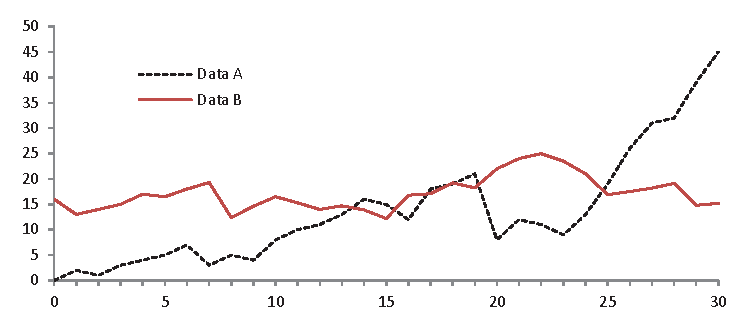
\includegraphics[width=\textwidth]{fig1.eps}
    \caption{A figure caption is always placed below the illustration.
        Please note that short captions are centered, while long ones are
        justified by the macro package automatically.} \label{fig1}
\end{figure}

\begin{theorem}
    This is a sample theorem. The run-in heading is set in bold, while
    the following text appears in italics. Definitions, lemmas,
    propositions, and corollaries are styled the same way.
\end{theorem}
%
% the environments 'definition', 'lemma', 'proposition', 'corollary',
% 'remark', and 'example' are defined in the LLNCS documentclass as well.
%
\begin{proof}
    Proofs, examples, and remarks have the initial word in italics,
    while the following text appears in normal font.
\end{proof}
For citations of references, we prefer the use of square brackets
and consecutive numbers. Citations using labels or the author/year
convention are also acceptable. The following bibliography provides
% a sample reference list with entries for journal
% articles~\cite{ref_article1}, an LNCS chapter~\cite{ref_lncs1}, a
% book~\cite{ref_book1}, proceedings without editors~\cite{ref_proc1},
% and a homepage~\cite{ref_url1}. Multiple citations are grouped
% \cite{ref_article1,ref_lncs1,ref_book1},
% \cite{ref_article1,ref_book1,ref_proc1,ref_url1}.
% %
% ---- Bibliography ----
%
% BibTeX users should specify bibliography style 'splncs04'.
% References will then be sorted and formatted in the correct style.
%
\bibliographystyle{splncs04}
\bibliography{references}

\end{document}
